\documentclass{beamer}
\usepackage[utf8]{inputenc}
\usepackage{listings}
\usepackage{booktabs}
\usepackage{amssymb}
\usepackage{nicefrac}
\usepackage{amsmath}
\usepackage{bbm}
\usepackage{bm}
\usepackage{enumitem}
\usepackage{hyperref}
\usepackage[export]{adjustbox}
\usepackage{svg}

\usetheme{Madrid}
\definecolor{mlpblue}{rgb}{0.1, 0.14, 0.24}

\useoutertheme{infolines} % Alternatively: miniframes, infolines, split
\useinnertheme{circles}
\usecolortheme[named=mlpblue]{structure}

\DeclareMathOperator{\Tr}{Tr}
\DeclareMathOperator{\Cov}{Cov}
\DeclareMathOperator{\Concat}{Concat}

\DeclareMathOperator*{\argmax}{arg\,max}
\DeclareMathOperator*{\argmin}{arg\,min}
\DeclareMathOperator*{\indep}{\perp \!\!\! \perp}

\lstset{basicstyle=\footnotesize\ttfamily,breaklines=true}

%------------------------------------------------------------
%This block of code defines the information to appear in the
%Title page
\title[Deep Neural Collapse]{Deep Neural Collapse:\thanks{\href{https://arxiv.org/abs/2206.04041}{Kothapalli.~[TMLR 2023]}}}

\subtitle{4 empirical metrics that identify population risk minimizers\thanks{\href{https://arxiv.org/abs/2012.05420}{E, Wojtowytsch. [PMLR 2022]}}}

\author[ECE ML Reading Group] % optional
{J.~Setpal} 

\date{November 13, 2024}

% \titlegraphic{
\includegraphics[width=7cm]{../shared/logo-long.pdf}}

%End of title page configuration block
%------------------------------------------------------------

%The next block of commands puts the table of contents at the 
%beginning of each section and highlights the current section:

\AtBeginSection[]
{
  \begin{frame}
    \frametitle{Outline}
    \tableofcontents[currentsection]
  \end{frame}
}
% ------------------------------------------------------------


\begin{document}

\frame{\titlepage}


%---------------------------------------------------------
% This block of code is for the table of contents after
% the title page
\begin{frame}
\frametitle{Outline}
\tableofcontents
\end{frame}
%---------------------------------------------------------

\section{Background \& Intuition}
\begin{frame}{Primer -- Support Vector Machines (SVMs)}
	\begin{columns}
		\begin{column}{.5\textwidth}
			~~We start with a linear SVM:
			\begin{center}
				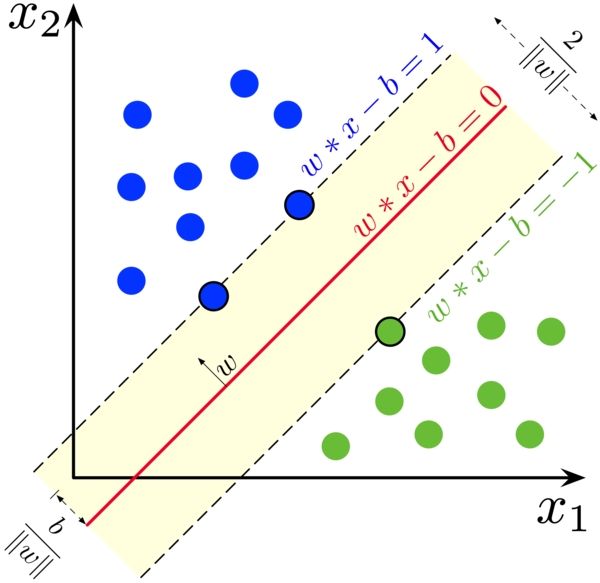
\includegraphics[width=\textwidth]{img/svm.png}
			\end{center} \pause
		\end{column}
		\hspace{1em}
		\begin{column}{.5\textwidth}
			An approach to obtain a non-linear decision boundary is to learn a hyperplane in higher-dimensions:
			\begin{center}
				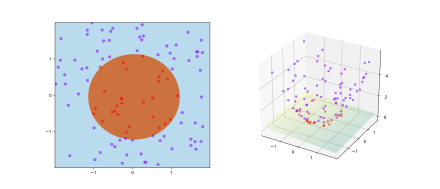
\includegraphics[width=\textwidth]{img/kernel.png}
			\end{center} \pause
			``Lazy'' approaches to kernel choices include \textit{polynomial} / \textit{RBF} kernels. \pause \newline \\

			The ``laziest'' kernel of all is a \textbf{deep neural network}.
		\end{column}
	\end{columns}
\end{frame}

\begin{frame}{Neural Networks are Incredibly Overparameterized}
	Our study today is constrained to classifiers. \pause WLOG, we can constrain our study to \textbf{image classifiers}.
	\begin{figure}[H]
		\centering
		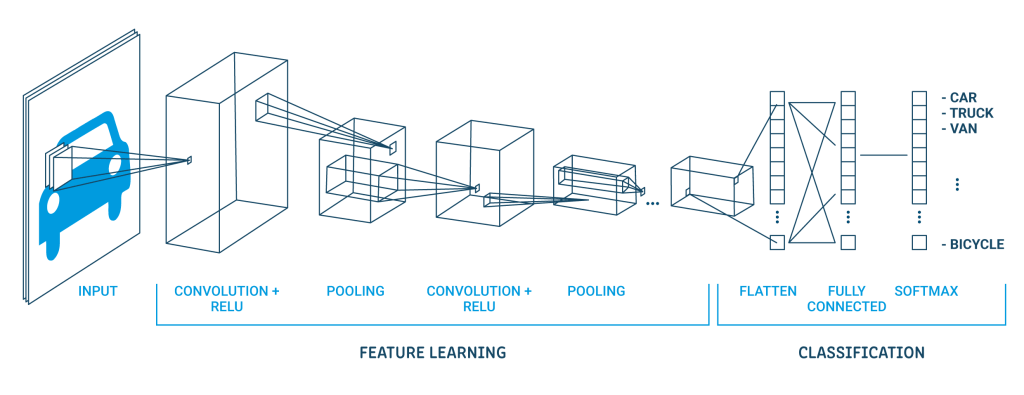
\includegraphics[width=\textwidth]{img/cnn.png}
	\end{figure} \pause

	\vspace{-1em}

	\textit{Traditional} Learning: $n \geq d;\ W \in \mathbb{R}^d,\ \mathcal{D} = \{(x_i, y_i)\}^n_{i=1}$ \pause \\
	\textit{Overparameterized} Learning: $d \geq n$ \pause \newline \\

	\textbf{Q}: Why does overparameterized learning generalize?
\end{frame}

\section{Conditions for Neural Collapse}
\begin{frame}{What is Deep Neural Collapse (DNC)?}
	\textbf{Deep Neural Collapse} is a phenomenon describing \textit{rigidity} in the feature representation(s) of the final layer(s) of \textit{overtrained} Deep Neural Networks. \pause \newline \\

	\textbf{Q${}_1$}: What does \textit{overtrained} mean? \\
	\textbf{A${}_1$}: When a sufficiently expressive network $h$ trained to minimize $\mathcal{L}(S_n)$ satisfies $h(x_i) = y_i\ \forall i$, it reaches the \textbf{Terminal Point of Training}. When trained beyond this point, the model is  \underline{overtrained}. \pause \newline \\

	\textbf{Q${}_2$}: What does \textit{rigidity} mean? \\
	\textbf{A${}_2$}: We quantify \textit{rigidity} by \underline{4 key metrics}, which iff satisifed, implies DNC. \pause \newline \\

	\textbf{Q${}_{2_a}$}: What are the 4 key metrics? \\
	\textbf{A${}_{2_a}$}: We'll talk about this next.
\end{frame}

\begin{frame}{$NC1$ -- Collapse of Variability $(\nicefrac{1}{2})$}
	At a high level, the structure of the penultimate layer collapses towards:
	\begin{figure}[H]
		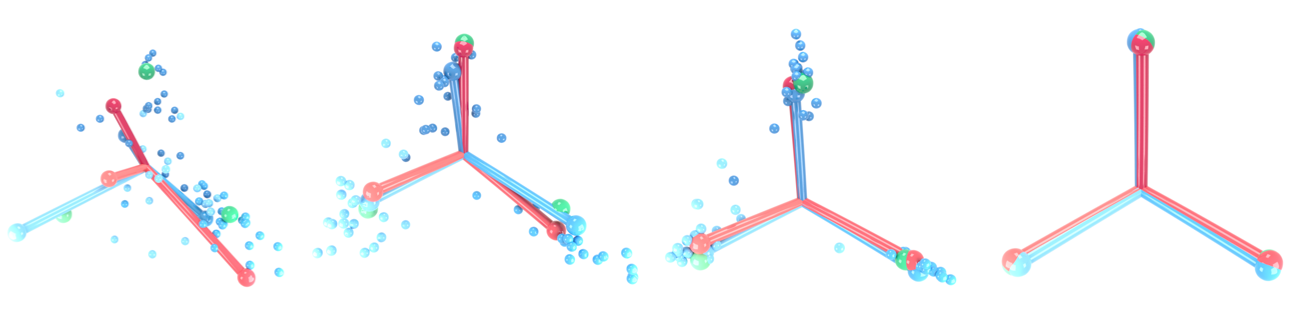
\includegraphics[width=\textwidth]{img/nc.png}
		\small Evolution of penultimate layer outputs on VGG13 trained on CIFAR10.
	\end{figure} \pause
	
	For all classes $k \in [K]$, datapoints $i \in [n]$ \underline{within a class}, \& penultimate feature vector $f(k, i)$,\pause~we have class-specific \& global means:
	\begin{gather}
		\bm{\mu}_k = \frac{1}{n} \sum^n_{i=1} f(k, i) \\
		\bm{\mu}_G = \frac{1}{K} \sum^K_{i=1} \bm{\mu}_k
	\end{gather}
\end{frame}
	
\begin{frame}{$NC1$ -- Collapse of Variability $(\nicefrac{2}{2})$}
	We can use them to calculate \textit{intra} and \textit{inter}-class differences:
	\begin{gather}
		\Cov_W = \frac{1}{Kn} \sum^K_{k=1} \sum^n_{i=1} ((f(k,i) - \bm{\mu}_{k})(f(k,i) - \bm{\mu}_{k})^T) \in \mathbb{R}^{m \times m} \\
		\Cov_B = \frac{1}{K} \sum^K_{k=1} ((\bm{\mu}_{k} - \bm{\mu}_G)(\bm{\mu}_{k} - \bm{\mu}_G)^T) \in \mathbb{R}^{m \times m}
	\end{gather} \pause
	Which we combine to measure overall \textbf{variability collapse}:
	\begin{gather}
		NC1 := \frac{1}{K} \Tr\left( \Cov_W \Cov_B^{\dagger} \right)
	\end{gather}
\end{frame}

\begin{frame}{Aside: Psuedoinverses}
	The \textbf{inverse} of a matrix $A$ is defined s.t.~it satisfies the following condition:
	\begin{gather}
		A, B, I \in \mathbb{R}^{d \times d} \text{ s.t. } AB = BA = I_d;\ B := A^{-1},\ A := B^{-1}
	\end{gather} \pause
	What about when $X \in \mathbb{R}^{n \times m}$? \pause A \textbf{psuedoinverse} is a \textit{generalized inverse}, which instead satisfies the following four conditions:
	\begin{gather}
		XX^{-1}X = X \\
		X^{-1}XX^{-1} = X^{-1} \\
		(XX^{-1})^{*} = XX^{-1} \\
		X^{-1}X^{*} = X^{-1} X
	\end{gather}
	Where $X^{*}$ is the conjugate transpose of $X$. \pause \newline \\

	\textbf{Implication:} We can compute correlation b/w general matrix dimensions.
\end{frame}

{\let\oldfootnoterule\footnoterule
\def\footnoterule{\only<2->\oldfootnoterule}
\begin{frame}{$NC2$ -- The Simplex ETF $(\nicefrac{1}{2})$}
	This time, we can on focus the \textbf{structure} of the class means:
	\vspace{-.5em}
	\begin{figure}[H]
		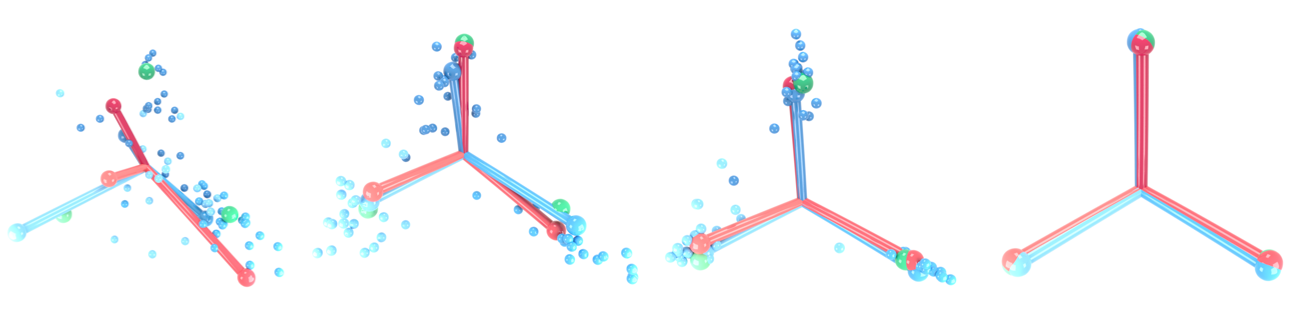
\includegraphics[width=\textwidth]{img/nc.png}
	\end{figure} \pause
	\vspace{-1em}
	A useful analogy is \textit{VSEPR}\footnote<2->{I sincerely apologize for making this reference.} from Chemistry. \pause Each class (atom) repels the other creating a \textbf{simplex equiangular tight frame} (simplex ETF). \pause
	\begin{itemize}[label=-]
		\item \textbf{Simplex} is the simplest polytope (object with flat sides). \pause
		\item \textbf{Equiangular Tight Frame} is a matrix $M \in \mathbb{R}^{K \times m}$ s.t.
			\vspace{-.5em}
			\begin{gather}
				|\langle \bm{m}_j, \bm{m}_k \rangle| = \alpha \ \exists \alpha \geq 0\ \forall j,k \text{ s.t. } j \neq k \\
				MM^{T} = \sqrt{\frac{C}{C-1}} \left(I_C - \frac{1}{C} \mathbbm{1}_{C \times C} \right)
			\end{gather}
			\vspace{.5em}
			Satisfying equiangular and tight respectively.
	\end{itemize}
\end{frame}
}

\begin{frame}{$NC2$ -- The Simplex ETF $(\nicefrac{2}{2})$}
	We can use this to define $NC2$. Given re-centered class means $\{\bm{\mu}_k - \bm{\mu}_G\}_{k \in [K]}$, they are \textbf{equidistant} if:
	\begin{gather}
		\| \bm{\mu}_k - \bm{\mu}_G \|_2 = \| \bm{\mu}_{k'} - \bm{\mu}_G \|_2\ \forall k, k' \in [K]
	\end{gather} \pause
	We then normalize each feature vector to create our simplex ETF:
	\begin{gather}
		M = \Concat\left(\left\{\frac{\bm{\mu}_k - \bm{\mu}_G}{\| \bm{\mu}_k - \bm{\mu}_G \|_2} \in \mathbb{R}^m \right\}^{[K]}\right) \in \mathbb{R}^{K \times m}
	\end{gather} \pause
	$M$ is now compared to it's distance from the simplex ETF:
	\begin{gather}
		NC2 := \left\| \underbrace{\frac{MM^T}{\| MM^T \|_F}}_{\text{feature vector as a simplex}} - \underbrace{\frac{1}{\sqrt{K - 1}} \left(I_K - \frac{\mathbbm{1}_{K \times K}}{K} \right)}_{\text{canonical simplex}} \right\|_F
	\end{gather}
	Setting up our second metric.
\end{frame}

\begin{frame}{$NC3$ -- Self-Dual Alignment}
	The final layer's weights $W \in \mathbb{R}^{K \times m}$ align with simplex ETF of $M$:
	\begin{gather}
		\frac{A}{\|A\|_F} \propto \frac{M}{\| M \|_F}
	\end{gather} \pause
	We can use this to setup the third metric:
	\begin{gather}
		NC3 := \left\| \underbrace{\frac{AM^T}{\| AM^T \|_F}}_{\equiv \text{ cosine similiarity}} - \underbrace{\frac{1}{\sqrt{K - 1}} \left(I_K - \frac{\mathbbm{1}_{K \times K}}{K} \right)}_{\text{canonical simplex}} \right\|_F
	\end{gather}
\end{frame}

\begin{frame}{$NC4$ -- Secretly $k$-NN}
	Finally, we observe that for $x_{n+1}$, the classification result $\equiv$ $k$-NN rule:
	\begin{gather}
		\argmax \hat{y}_{n+1} = \argmin_{k \in [K]} \| f(x_{n+1}) - \bm{\mu}_k \|_2
	\end{gather} \pause
	Which we can use to setup our final metric:
	\begin{gather}
		NC4: \frac{1}{Kn} \sum^K_{k=1} \sum^n_{i=1} \mathbbm{1}\left[\argmax \hat{y}_{i} \neq \argmin_{k \in [K]} \| f(x_{i}) - \bm{\mu}_k \|_2\right]
	\end{gather} \pause

	If each of the 4 previous metrics $\rightarrow 0$, the network is considered \textbf{collapsed}.
\end{frame}

\section{Optimality of Neural Collapse}
\begin{frame}{Modelling Neural Collapse}
	\textbf{Unconstrained Features Model}: To maintain the expressivity of $\mathcal{H}$, properties NC is studied by treating $f_i, i \in \{1, \ldots, L-1\}$ as \textit{free optimization parameters}:
	\begin{center}
		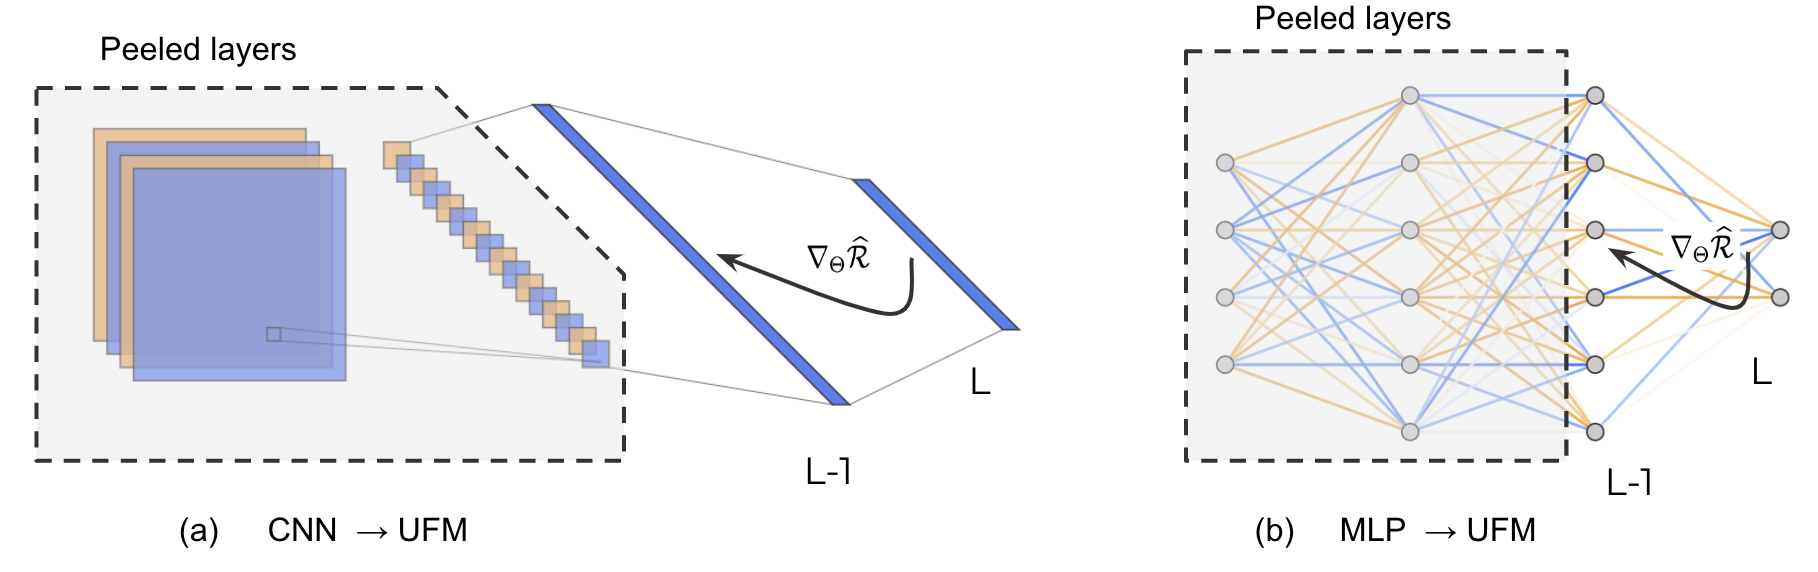
\includegraphics[width=\textwidth]{img/ufm.png}
	\end{center}
	\vspace{-1.5em}
	\begin{gather}
		h_L(x) = A \underbrace{f_{1:L-1}(x)}_{NC} + b
	\end{gather} \pause
	We can further discuss the ideal values of $A, f, b$ and training dynamics (regularization, loss functions, normalization) that encourage it.
\end{frame}

\begin{frame}{Do We Even Want This? -- Data Independence}
	Here's what the metric convergence plots look like, with \textit{random labels}.
	\begin{figure}[H]
		\centering
		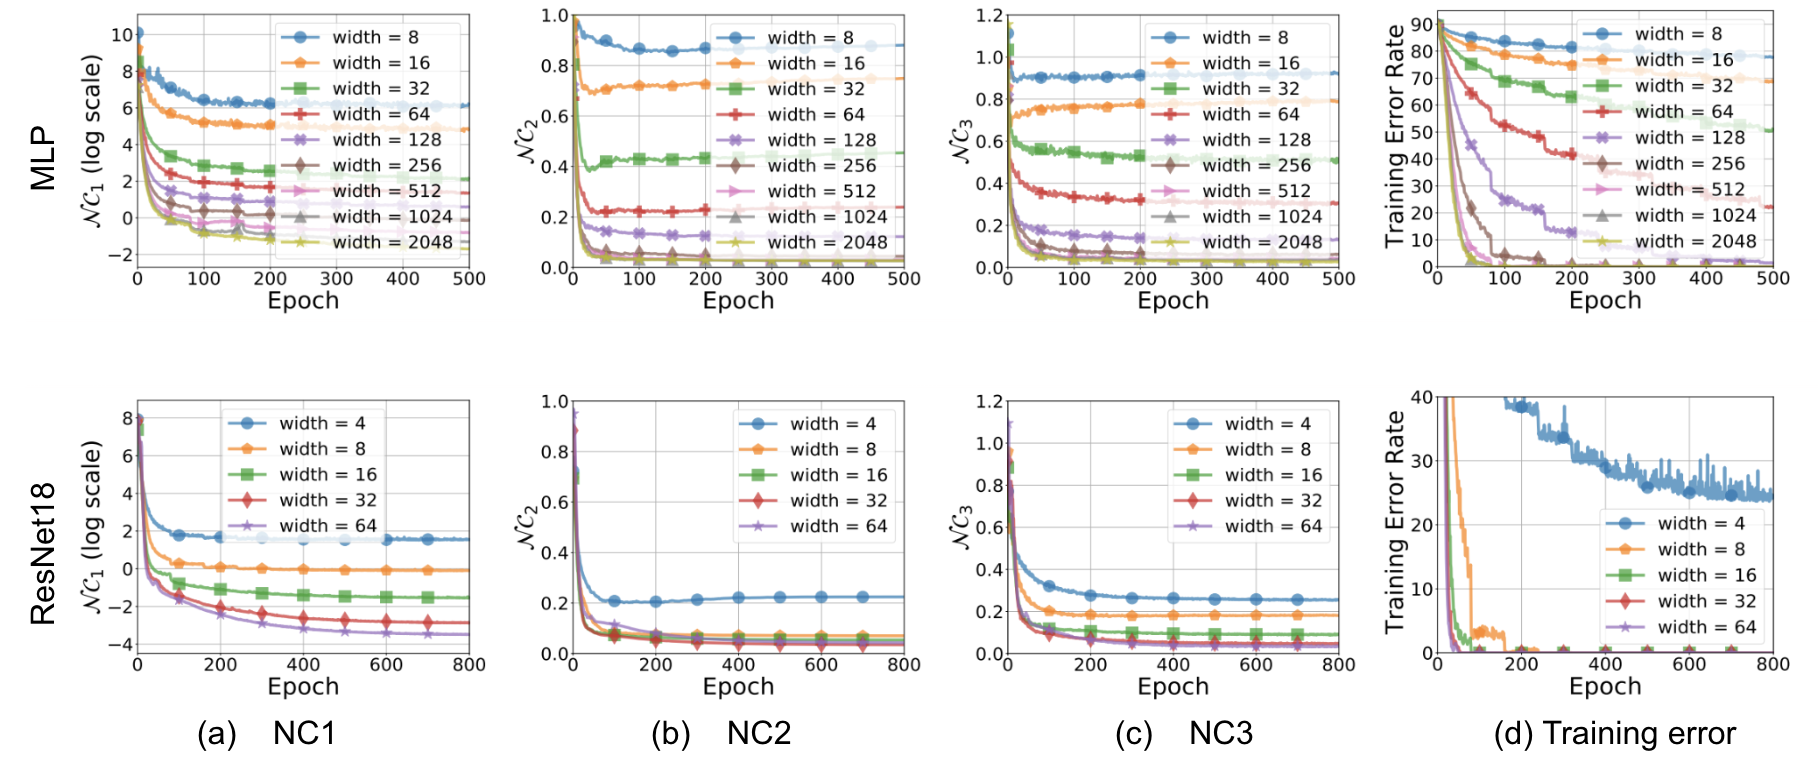
\includegraphics[width=.78\textwidth]{img/nc_random_labels.png}
	\end{figure} \pause
	\vspace{-1em}
	\textbf{Q}: Do we even want this? \pause \\
	\textbf{A}: Yes. Here's some reasons why:
	\begin{enumerate}[label=\arabic*.]
		\item \textbf{OOD}: \{NC1, NC2, NC3\} $\gg 0$ imply unconfident predictions. \pause
		\item \textbf{Forced ETF}: The final layer can be a fixed as a simplex. \pause
		\item \textbf{Data dependenent explanation}: AGOP induces NC.
	\end{enumerate}
\end{frame}

\begin{frame}{Optimality of NC (Softmax-CE Loss)}
	Softmax CE is defined element-wise as follows:
	\begin{gather}
		\Phi(z)_j = -\log \frac{\text{exp}(z_j)}{\sum^k_{i=1}\text{exp}(z_i)} = \log \sum^k_{i=1}\text{exp}(z_i) + \log \text{exp}(z_j)
	\end{gather}
	is convex $\forall j \in \{1, \ldots, k\}$. \pause
	\begin{gather}
		z_k := \frac{1}{n} \int_{C_k} h(x) \mathbb{P}(dx) \\
		\int_{C_k} \Phi_k(h(x)) \mathbb{P}(dx) \geq
		\int_{C_k} \Phi_k(z_k) \mathbb{P}(dx)
	\end{gather} \pause
	
	Consequently, we have that:
	\begin{gather}
		\mathcal{R}(\bar{h}) \leq \min_{h \in \mathcal{H}} \mathcal{R}(h)
	\end{gather}
	Establishing NC describing the optimal geometry within the final layer for \textit{population} risk minimization.
\end{frame}

\begin{frame}{Thank you!}
	\begin{center}
		Have an awesome rest of your day!
	\end{center}
	\begin{center}
		\textbf{Slides:} \url{https://cs.purdue.edu/homes/jsetpal/slides/dnc.pdf}
	\end{center}
\end{frame}

\end{document}
